\documentclass{standalone}
\usepackage{pgfplots}
\pgfplotsset{compat=newest}

\begin{document}
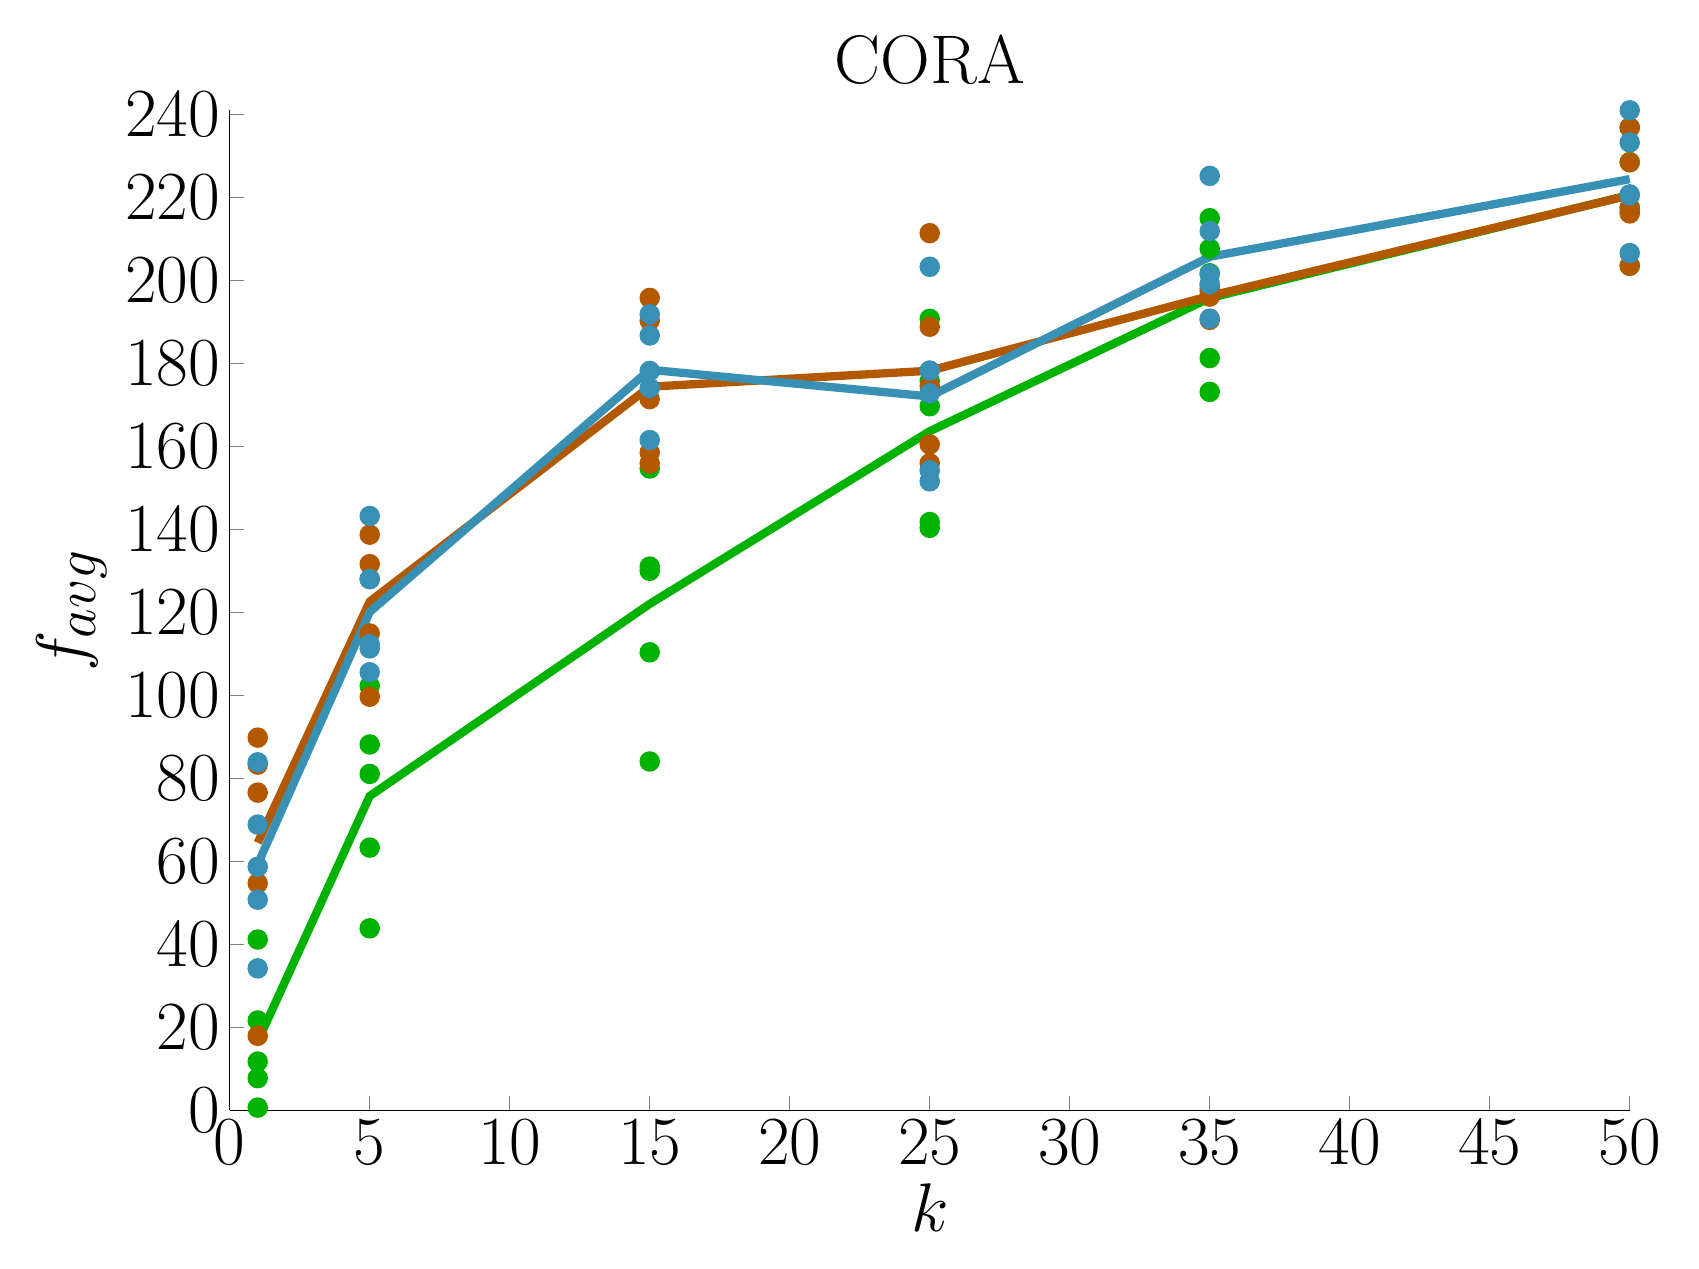
\begin{tikzpicture}

\begin{axis}[%
title style={font=\Huge},
title=CORA,
tick label style={font=\Huge},
label style={font=\Huge},
legend style={font=\Huge},
view={0}{90},
max space between ticks=50pt,
width=7in,
height=5in,
scale only axis,
xmin=0, xmax=50,
%xtick={0, 20, 40, 60, 80, 100},
xlabel={$k$},
ymin=0, ymax=240.95,
ylabel={$f_{avg}$},
major tick length=5pt,
axis lines*=left,
legend cell align=left,
clip=false]

\addplot [
only marks,
mark=*,
mark size=3.5pt,
color=green!70!black,
%solid,
%line width=2pt,
]
coordinates{
(1,0.65)(1,7.75)(1,11.75)(1,21.65)(1,41.15)(5,43.85)(5,63.3)(5,81.05)(5,88.15)(5,102.25)(15,84.05)(15,110.35)(15,130.0)(15,131.0)(15,154.65)(25,140.35)(25,141.75)(25,169.65)(25,175.65)(25,190.7)(35,173.1)(35,181.25)(35,201.7)(35,207.6)(35,214.95)(50,203.5)(50,216.5)(50,217.5)(50,228.45)(50,236.8)
};

\addplot [
only marks,
mark=*,
mark size=3.5pt,
color=orange!70!black,
%solid,
%line width=2pt,
]
coordinates{
(1,17.95)(1,54.7)(1,76.55)(1,83.3)(1,89.8)(5,99.65)(5,114.9)(5,128.0)(5,131.6)(5,138.7)(15,155.85)(15,158.5)(15,171.35)(15,190.3)(15,195.75)(25,155.9)(25,160.45)(25,174.5)(25,188.8)(25,211.35)(35,190.45)(35,196.05)(35,197.4)(35,198.05)(35,199.1)(50,203.5)(50,216.1)(50,217.5)(50,228.45)(50,236.8)
};

\addplot [
only marks,
mark=*,
mark size=3.5pt,
color=cyan!70!black,
%solid,
%line width=2pt,
]
coordinates{
(1,34.2)(1,50.75)(1,58.7)(1,68.85)(1,83.85)(5,105.55)(5,111.3)(5,112.3)(5,128.0)(5,143.2)(15,161.5)(15,174.05)(15,178.15)(15,186.7)(15,191.8)(25,151.55)(25,154.2)(25,172.75)(25,178.25)(25,203.25)(35,190.75)(35,199.05)(35,201.45)(35,211.85)(35,225.15)(50,206.55)(50,220.45)(50,220.7)(50,233.2)(50,240.95)
};
p
\addplot [
color=green!70!black,
solid,
line width=3pt
]
coordinates{
(1,16.59)(5,75.72)(15,122.01)(25,163.62)(35,195.72)(50,220.55)
};

\addplot [
color=orange!70!black,
solid,
line width=3pt
]
coordinates{
(1,64.46)(5,122.57)(15,174.35)(25,178.2)(35,196.21)(50,220.47)
};

\addplot [
color=cyan!70!black,
solid,
line width=3pt
]
coordinates{
(1,59.27)(5,120.07)(15,178.44)(25,172.0)(35,205.65)(50,224.37)
};


\end{axis}
\end{tikzpicture}
\end{document}
